\subsection{The need for smoothing}
\label{sec:need for smoothing}
Let $\formula$ be an MTL formula with horizon $N$.
We aim to solve the following control problem $P_\rob$.
\begin{subequations}
\label{eq:general_ctrl}
\begin{align}
P_\rob:\, \max\, & \rob_{\formula}(\sstraj) - \gamma \sum_{k=0}^{N-1} l(x_{k+1},u_{k}) \label{eq:general ctrl obj}\\
\text{s.t. } & x_{k+1} = f(x_k,u_k), \, \forall k=0,\dotsc,N-1 \label{eq:general ctrl dyn}\\
 & x_k \in X, \, \forall k=0,\dotsc,N \label{eq:general ctrl X}\\
 & u_k \in U, \, \forall k=0,\dotsc,N-1 \label{eq:general ctrl U}\\
 & \delta \rob_{\formula}(\sstraj) \geq \delta \epsilon_{\text{Meyer}} \label{eq:general ctrl pos rob}
\end{align}
\end{subequations}

We want to use established, powerful gradient descent algorithms \cite{Polak97_Optim}, rather than heuristics like Simulated Annealing \cite{kirkpatrickV_SA83}. 
In the above formulation, $l(x_{k+1},u_{k})$ is a system specific control cost, e.g. the LQR cost $x_k'Qx_k + u_k'Ru_k$. $\gamma \geq 0$ is weighting parameter, which is a design choice. $X$ and $U$ define constraints on the state $x$ and control $u$ respectively. $f$ represents the dynamical system, with $x$ as the state and $u$ as inputs. Finally, the last constraint enforces $\rob \geq 0$, i.e. the specification is satisfied. 
$\delta$ here is a binary design choice, $1$ if the constraint is meant to be enforced, $0$ otherwise.

Gradient descent algorithms typically offer convergence guarantees to the function's minima and offer advantages which were reviewed in Sec. \ref{sec:intro}.
%have known convergence rates for certain function classes, and have been optimized so they outperform heuristics that don't have access to the objective's gradient information.
%Moreover, they usually have a fewer parameters to be set by the user, and important issues like step-size selection are rigorously addressed.

To apply gradient descent methods, we require a differentiable objective function. 
Our objective function, $\robf$, is non-differentiable, because it uses the distance, max, and min functions, all of which are non-differentiable.
One may note that these functions are all differentiable almost everywhere (a.e.) on their domain.
That is, the set of points in their domain where they are non-differentiable has measure 0 in $\Re^n$. 
Therefore, by measure additivity, the composite function $\robf$ is itself differentiable almost everywhere.
Thus, one may be tempted to `ignore' the singularities (points of non-differentiability), and apply gradient descent to $\robf$ anyway.
The rationale for doing so is that sets of measure 0 are unlikely to be visited by gradient descent, and thus don't matter. 
However, as we show in the next example, the lines of singularity (along which the objective is non-differentiable) can be  precisely the lines along which the objective increases the fastest.
See also \cite{Cortes08_Discontinuous}.
Thus they are consistently visited by gradient descent, after which it fails to converge because of the lack of a gradient.


\begin{exmp}
	\label{ex:cluster nondiff}
	A simple example illustrates how gradient descent gets stuck at singularities. We use the optimization algorithm Sequential Quadratic Programming (SQP) \cite{Polak97_Optim} to maximize the robustness of $\formula = \neg (x \in U)$, where $U=[-1,1]^2$ is the unsafe red square in Fig.~\ref{fig:DumbExample}.
	In this case, $\robf$ is simply $\dist(x_0,U)$, the distance of the first trajectory point to the set.
	The search space is $[-2.5,2.5]^2$ (big grey square in Fig. \ref{fig:DumbExample}). 
	The most robust point is $x^* = [2.5,2.5]$ (green `+' in figure), being furthest from the unsafe set.
	We initialize the SQP at $x_0=[0,0]$. 
	SQP generates iterates (blue circles) \textit{on the line of singularity} connecting $[1,1]$ to $x^*$ and ultimately gets stuck at $x=[1,1]$.
	That's because along the line, the gradient does not exist and attempts by SQP to approximate it numerically fail, prompting it to generate smaller and smaller step-sizes for the approximation.
	Ultimately, SQP aborts due to the step-size being too small, and concludes it is at a local minimum.
\end{exmp}	
\begin{figure}[t]
\centering
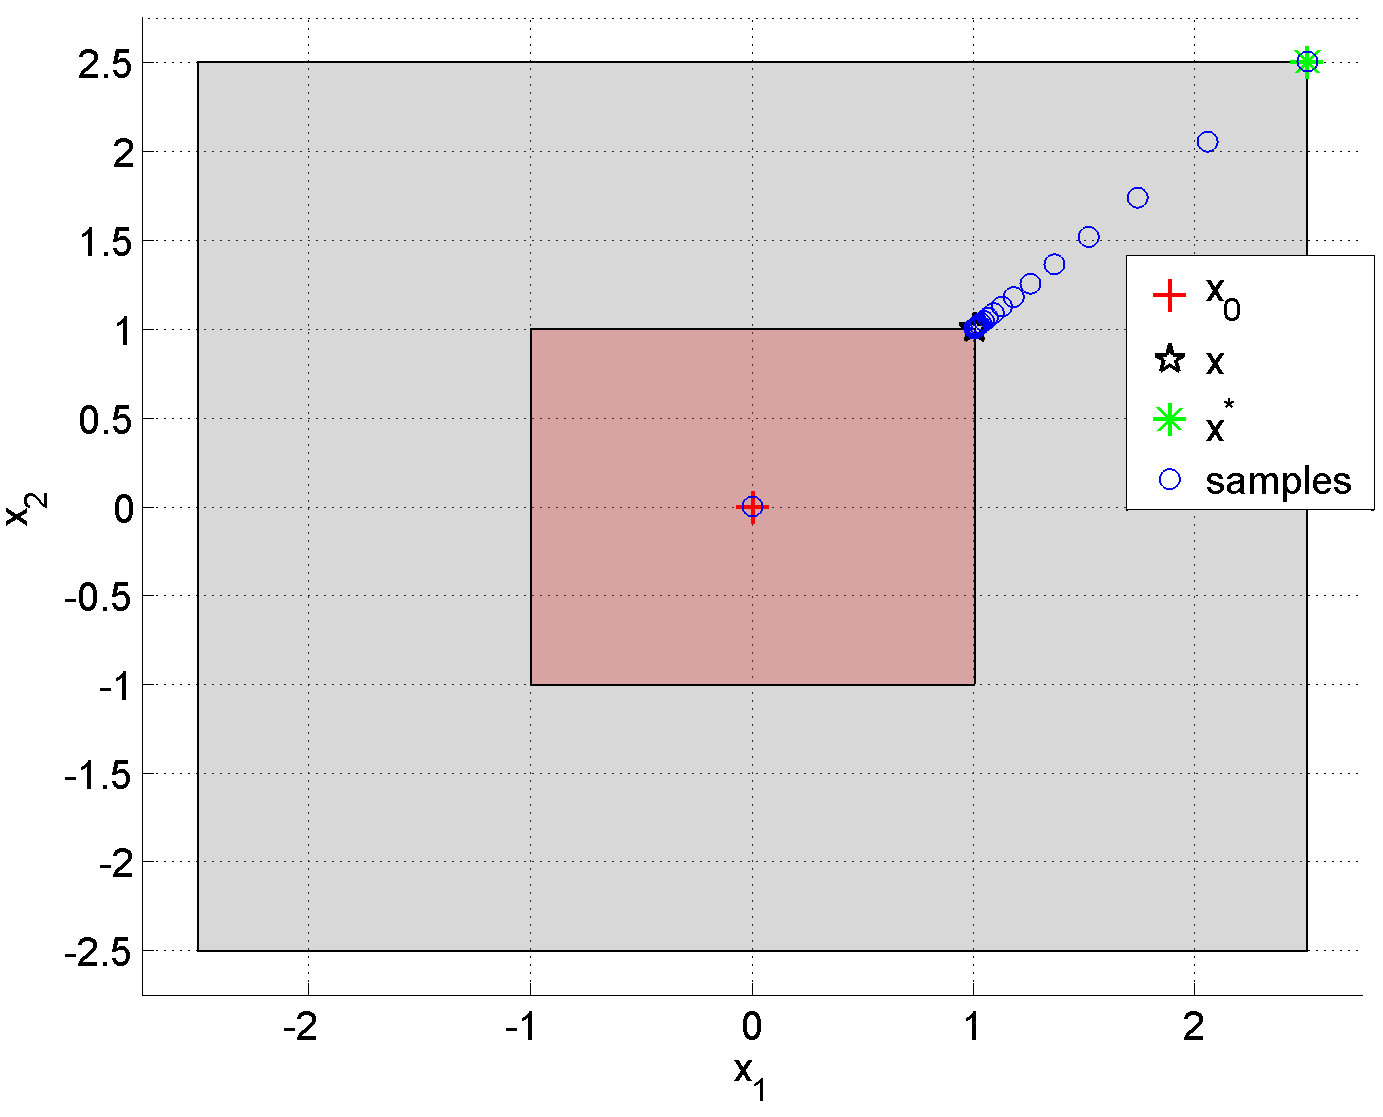
\includegraphics[width=0.49\textwidth]{figures/DumbOptEx_scissored}
\vspace{-20pt}
\caption{{\small Iterates of SQP for Example \ref{ex:cluster nondiff}. Colors in online version.}}
\vspace{-10pt}
\label{fig:DumbExample}
\end{figure}


